\documentclass[12pt,a4paper]{article}

\setlength{\topmargin}{0.0in}
\setlength{\oddsidemargin}{0.33in}
\setlength{\textheight}{9.0in}
\setlength{\textwidth}{6.0in}
\renewcommand{\baselinestretch}{1.25}



\usepackage{hyperref}
% \usepackage[utf8]{inputenc}
% \usepackage[T1]{fontenc}
\usepackage{float}
\usepackage{enumitem}
\usepackage{listings}
\usepackage{amsmath}
\usepackage{amssymb}
\usepackage{amsthm}
\usepackage{tikz}
\usetikzlibrary{decorations.pathreplacing}
\usepackage{amsfonts}
\usepackage{graphicx}
\usepackage{longtable}
\usepackage{booktabs}
\usepackage{mathtools}
\usepackage{subcaption}
\usepackage{caption}
\newcommand{\dv}[2]{\frac{\mathrm{d} #1}{\mathrm{d} #2}}
\usepackage{caption}
\captionsetup[figure]{font=small} 
% \captionsetup[table]{font=small}
\usepackage[capitalize,nameinlink]{cleveref}
\usepackage{mathtools}
\newcommand{\defeq}{\vcentcolon=}
\newcommand{\eqdef}{=\vcentcolon}
\usepackage{amsmath}
\usetikzlibrary{arrows.meta}

\definecolor{meshOrange}{RGB}{238,145,0}
\definecolor{cellGreen}{RGB}{135,220,20}
\definecolor{eigenPurple}{RGB}{155,0,190}
\definecolor{axisGray}{RGB}{75,85,85}

% Define environments
% \newtheorem{theorem}{Theorem}
% \newtheorem{definition}{Definition}
% \newtheorem{lemma}{Lemma}
% \newtheorem{corollary}{Corollary}


\newtheoremstyle{boldthm}
  {3pt}        % space above
  {3pt}        % space below
  {\itshape}   % body font
  {}           % indent
  {\bfseries}  % theorem head font
  {.}          % punctuation
  {.5em}       % space after theorem head
  {\thmname{#1}\thmnumber{ #2}\thmnote{ \textbf{(#3)}}}

\newtheoremstyle{bolddefn}
  {3pt}
  {3pt}
  {\itshape} 
  {}
  {\bfseries}
  {.}
  {.5em}
  {\thmname{#1}\thmnumber{ #2}\thmnote{ \textbf{(#3)}}}


\theoremstyle{boldthm}
\newtheorem{theorem}{Theorem}[section]
\newtheorem{corollary}[theorem]{Corollary}
\newtheorem{lemma}[theorem]{Lemma}
\newtheorem{proposition}[theorem]{Proposition}

\theoremstyle{bolddefn}
\newtheorem{definition}[theorem]{Definition}
\newtheorem{example}[theorem]{Example}
\newtheorem{remark}[theorem]{Remark}



\title{Formulating the Outer Loop}
\author{}
\date{}

\begin{document}

\maketitle

\section{Matt's Algorithm: A Quick Review}

Recall that 
\begin{equation}
\begin{aligned}
    \gamma(z, A) &= \min \{ \sigma_{\text{inf}}(A-zI), \sigma_{\text{inf}}((A-zI)^*) \} \\
    &= \| (A-zI)^{-1} \|^{-1}.\\
\end{aligned}
\end{equation}
In Matt's algorithm for pseudospectra, we compute values of $\Phi_n(z, A)$ that converge to $\gamma(z, A)$ from above, i.e., 
\begin{equation} \label{lim}
    \lim_{n\rightarrow \infty} \sup_{z \in K} | \Phi_n(z, A) - \gamma(z, A) | = 0 \qquad \forall \text{ compact sets } K \in \mathbb{C},
\end{equation}
and
\begin{equation} \label{above}
    \gamma(z, A) \le \Phi_n(z, A) \qquad \forall \text{ sufficiently large } n.
\end{equation}
Thus, to compute the $\epsilon$-pseudospectrum, we compute $\Phi_n(z, A)$ for each $z \in \text{Grid}(n)$ (grid over the complex plane) and retain all the values for which $\Phi_n(z, A) < \epsilon.$

To achieve this with operator folding, we consider the Rayleigh quotients
\begin{equation}
    R_{z, A}^{(1)}(f) = \frac{\| (A-zI) f \|^2}{\|f\|^2}, 
\end{equation}
and 
\begin{equation}
    R_{z, A}^{(2)}(f) = \frac{\| (A-zI)^* f \|^2}{\|f\|^2},
\end{equation}
and notice that
\begin{equation}
    \gamma(z, A) = \sqrt{ \min \left\{ \inf_{f \in D(A) \setminus \{0\}} R_{z, A}^{(1)}(f) , \inf_{f \in D(A^*) \setminus \{0\}} R_{z, A}^{(2)}(f) \right\}}.
\end{equation}
To approximate $\gamma(z, A)$ in a way that respects \eqref{lim} and \eqref{above}, we truncate the Rayleigh quotients and take
\begin{equation}
    \Phi_n(z, A) = \sqrt{ \min\{a, b\} },
\end{equation}
where 
\begin{equation}
    a = \frac{x^* L_n^{(1)}(z) x}{x^* G_n x},
\end{equation}
and
\begin{equation}
    b = \frac{x^* L_n^{(2)}(z) x}{x^* G_n x},
\end{equation}
where, 
\begin{equation}
    [L_n^{(1)}(z)]_{i,j} = ( (A-zI) e_j, (A-zI) e_i ), \qquad 1 \le i, j \le n,
\end{equation}
\begin{equation}
    [L_n^{(2)}(z)]_{i,j} = ( (A-zI)^* e_j, (A-zI)^* e_i ), \qquad 1 \le i, j \le n,
\end{equation}
\begin{equation}
    [G_n]_{i,j} = ( e_j, e_i ), \qquad 1 \le i, j \le n,
\end{equation}
for a complete and linearly independent set of vectors $\{e_j\}_{j \in \mathbb{N}},$ whose linear span is a core of $A$ and $A^*.$ 

Notice that the folded operators, namely, $(A-zI)^*(A-zI)$ and $(A-zI)(A-zI)^*,$ are self-adjoint nonnegative operators. As Matt claims, ``No assumption is made about the bottom of the spectrum of these
operators being discrete. Computing the bottom of the spectrum of non-negative self-adjoint
operators is typically much easier than other parts of the spectrum, and less prone to the
discretisation pitfalls." 

\section{Folded Eigenproblems Using the FEM}

When using the finite element method to compute $\Phi_n(z, A),$ we formulate the generalized folded eigenproblems as the following variational problems: 
\begin{equation}
    \text{Find } (u, \lambda_a) \text{ such that } ((A-zI)u, (A-zI)v) = \lambda_a (u, v) \text{ for all } v \in V,
\end{equation}
\begin{equation}
    \text{Find } (u, \lambda_b) \text{ such that } ((A-zI)^*u, (A-zI)^*v) = \lambda_b (u, v) \text{ for all } v \in V.
\end{equation}
As per usual, we compute the Galerkin approximations of the solutions of these eigenproblems, i.e., we consider a finite-dimensional subset $V_h \subset V$ and we approximate the solution of the following problems: 
\begin{equation}\label{Gal1}
    \text{Find } (u_h, \lambda_{a,h}) \text{ such that } ((A-zI)u_h, (A-zI)v_h) = \lambda_{a,h} (u_h, v_h) \text{ for all } v_h \in V_h,
\end{equation}
\begin{equation}\label{Gal2}
    \text{Find } (u_h, \lambda_{b,h}) \text{ such that } ((A-zI)^*u_h, (A-zI)^*v_h) = \lambda_{b,h} (u_h, v_h) \text{ for all } v_h \in V_h.
\end{equation}
In doing so, we compute
\begin{equation}
    a_h = \min\{\lambda_{a, h} \text{ that satisfies \eqref{Gal1}}\}, \qquad b_h = \min\{\lambda_{b, h} \text{ that satisfies \eqref{Gal2}} \},
\end{equation}
and take
\begin{equation}
   \Phi_n(z, A) = \sqrt{ \min\{a_h, b_h\} }. 
\end{equation}



\section{DWR for Eigenvalues}

\subsection{The Rannacher and Bangerth Formulation}


Consider the following infinite-dimensional eigenproblem: find a $u \in V$ and a $\lambda \in \mathbb{C}$ such that
\begin{equation}
    Au = \lambda M u,
\end{equation}
where $A$ and $M$ are linear operators in the complex Hilbert space $V.$ The corresponding variational formulation is 
\begin{equation} \label{primal}
    a(u, \psi) = \lambda m(u, \psi) \qquad \forall \psi \in V,
\end{equation}
where $m(u, u)=1.$ The corresponding adjoint problem is to find the eigenpair $U^* = \{u^*, \lambda^*\}$ such that
\begin{equation} \label{dual}
   a(\phi, u^*) = \overline \lambda^* m(\phi, u^*) \qquad \forall \phi \in V, 
\end{equation}
where $m(u, u^*) = 1.$
In Chapter 7 of their text, Rannacher and Bangerth deduce the following result:


\begin{proposition}[Proposition 7.1 in Rannacher and Bangerth]
With the primal and dual eigenvalue residuals
\begin{equation}
\rho(u_h,\lambda_h)(\cdot)
:= a(u_h,\cdot) - \lambda_h m(u_h,\cdot),
\end{equation} 
\begin{equation}
\rho^*(u_h^*,\lambda_h^*)(\cdot)
:= a(\cdot,u_h^*) - \overline{\lambda_h^*} m(\cdot,u_h^*),
\end{equation}
we have the error representation
\begin{equation}\label{err}
\lambda - \lambda_h
=
\frac{1}{2}\rho(u_h,\lambda_h)(u^*-\psi_h)
+
\frac{1}{2}\rho^*(u_h^*,\lambda_h^*)(u-\varphi_h)
+
\mathcal{R}_h,
\end{equation}
for arbitrary $\psi_h,\varphi_h\in V_h$, with the cubic remainder term
\begin{equation}
\mathcal{R}_h
=
\frac{1}{2}(\lambda-\lambda_h)
m(u-u_h,u^*-u_h^*).
\end{equation}
\end{proposition}

When the operator $A$ is self-adjoint, as is the case for the folded operator eigenproblem, the error estimate becomes

\begin{proposition}[Symmetric Version of Proposition 7.1]
With the primal eigenvalue residual,
\begin{equation}
\rho(u_h,\lambda_h)(\cdot)
:= a(u_h,\cdot) - \lambda_h m(u_h,\cdot),
\end{equation} 
we have the error representation
\begin{equation}\label{err}
\lambda - \lambda_h
=
\rho(u_h,\lambda_h)(u-\psi_h)
+
\mathcal{R}_h,
\end{equation}
for arbitrary $\psi_h\in V_h$, with the remainder term
\begin{equation}
\mathcal{R}_h
=
\frac{1}{2}(\lambda-\lambda_h)
m(u-u_h,u-u_h).
\end{equation}
\end{proposition}

We note that in our computations, we do not have access to $u.$ Thus, to compute the error estimate, we compute an `enriched' approximation of $u,$ denoted $u_h^+ \in V_h^+,$ which is an approximation of $u$ in a `better' space than $V_h$ (due to a higher polynomial degree or to a finer mesh). Furthermore, by Galerkin orthogonality, we can suppress the subtraction of $\psi_h$ in the error estimate. However, when this error estimate is localized for adaptivity, it is common to take either $u - \psi_h \approx u_h^+ - I_h u_h^+,$ where $I_h$ interpolates $u_h^+$ onto $V_h,$ or $u - \psi_h \approx u_h^+ - u_h.$ In taking the former approach, the error estimate of interest is 
\begin{equation} \label{sym}
\lambda - \lambda_h
=
\rho(u_h,\lambda_h)(u_h^+-I_h u_h^+)
+
\mathcal{R}_h,
\end{equation} 
with the remainder term
\begin{equation} \label{R term}
\mathcal{R}_h
=
\frac{1}{2}(\lambda-\lambda_h)
\, m(u_h^+- I_h u_h^+,u_h^+- I_hu_h^+).
\end{equation}
Substituting \eqref{R term} into \eqref{sym}, and solving for $\lambda - \lambda_h$, we obtain
\begin{equation} \label{eta}
    \lambda - \lambda_h = \frac{\rho(u_h,\lambda_h)(u_h^+-I_h u_h^+) }{ 1 - \frac{1}{2} \,m(u_h^+- I_h u_h^+,u_h^+- I_hu_h^+) },
\end{equation}
which will serve as our DWR estimate for the eigenvalues of the folded operator eigenproblem.


\subsection{A Note on Multiplicity}

Assume that $A$ is a self-adjoint operator and use $F_z = (A-zI)^*(A-zI) = (A-zI)^2$ to denote the corresponding folded operator. When considering the smallest eigenvalue of the folded operator eigenproblem, i.e., $F_z u = \mu u,$ one must consider the possibility of a multiple eigenvalue. To see this, notice that if $(\lambda, u_i)$ satisfies $A u = \lambda u_i$ with multiplicity $q$ (and so $i=1, \dots q$), then $(\mu = (\lambda-z)^2, u_i)$ is an eigenpair of the folded operator for each $i=1, \dots, q.$ 

Let the $j$th eigenvalue of $A$ be denoted by $\lambda_j.$ The smallest eigenvalue of the folded operator is
\begin{equation}
    \mu_{\min}(z) = \min_j (\lambda_j-z)^2 .
\end{equation}
Thus, the smallest folded eigenvalue comes from whichever eigenvalue of $A$ is
closest to $z$.

If $\lambda_j$ is the unique eigenvalue of $A$ closest to $z$, then the
multiplicity of $\mu_{\min}(z)$ is just the multiplicity of $\lambda_j$.
For example, if $\lambda=3$ has multiplicity $2$, then $(3-z)^2$
has multiplicity $2$ as a folded eigenvalue. Thus, at, say, $z=3$, the
folded operator has a zero eigenvalue of multiplicity $2$.

Now suppose two nearby eigenvalues of $A$ are $\lambda_1=2,$ and $\lambda_2 = 3.$
Under the folded operator, these map to $(2-z)^2$ and $(3-z)^2,$ respectively.
If $z$ is closer to $2$, then $(2-z)^2$ is the smallest folded eigenvalue. If
$z$ is closer to $3$, then $(3-z)^2$ is the smallest folded eigenvalue.

However, a switch occurs at the midpoint, $z = \frac{2+3}{2} = 2.5,$ where
$(2-2.5)^2 = (3-2.5)^2.$
In this case, both eigenvalues of $A$ contribute to the same smallest folded eigenvalue and the eigenspace for $\mu_{\min}(z)$ contains the eigenspace for $\lambda_1$ and $\lambda_2,$ and the multiplicities add.

With this in mind, we must be aware that the smallest folded eigenvalue, which we will now refer to as $\lambda$ and its approximation $\lambda_h,$ may have multiplicity greater than one. The DWR error estimate for $\lambda - \lambda_h,$ as given by \eqref{eta}, requires a single $u_h$ and a corresponding $u_h^+.$ When $\lambda_h$ has multiplicity greater than one, $u_h$ and $u_h^+$ can approximate any linear combination of the eigenbasis corresponding to $\lambda.$ However, for the remainder term in the DWR error estimate to be small, and for the error estimate to be of use, we want to align $u_h$ and $u_h^+$ so that $u_h^+$ approximates the eigenfunction that $u_h$ would converge to as $h\rightarrow 0.$ To do so, we take a least-squares alignment approach. In particular, given the computed first folded eigenpair, $(\lambda_h, u_h),$ we compute the relevant cluster of eigenpairs in the enriched space $V_h^+.$ Then, to choose an eigenfunction in the enriched space that aligns with the specific $u_h$ in $V_h$, we solve a small least squares problem. In particular, if the cluster size is $k$ and the computed eigenbasis in $V_h^+$ is $\{u^+_{h,1},\ldots,u^+_{h,k}\},$ we seek coefficients \(x_1,\ldots,x_k\) that satisfy
\begin{equation}
    \min_{x_1,\ldots,x_k}
    \left\| u_h - \sum_{j=1}^k x_j u^+_{h,j} \right\|^2.
\end{equation}
Equivalently, we want to find the vector in
\begin{equation}
    \operatorname{span}\{u^+_{h,1},\ldots,u^+_{h,k}\}
\end{equation}
that is closest to \(u_h\). 


\section{DWR for $\Phi_n(z, A)$}

Now we want to use our DWR estimate for the error in the smallest folded eigenvalues to approximate the error in $\Phi_n(z, A).$ 


To do so, we first note that the DWR error estimate requires an eigenfunction. However, $\gamma(z, A)$ requires the bottom of the spectrum of the folded operators and $\Phi_n(z, A)$ approximates the bottom of the spectrum using truncated Rayleigh quotients. If the bottom of the spectra does not consist of an isolated eigenvalue of finite multiplicity, then there is no eigenfunction associated with the computed spectral value and the DWR error estimate does not make sense. To overcome this issue, we will (for now) assume that the bottom of the spectrum of each folded operator consists of an isolated eigenvalue with finite multiplicity (I still need to understand what conditions on $A$ guarentee this). Then, computing $\gamma(z,A)$ can be thought of as finding the first eigenpair of two infinite-dimensional eigenproblems (instead of finding the  bottom of the spectrum) and computing $\Phi_n(z,A)$ can be thought of as finding the first eigenpair of the truncated eigenproblems. In this case, a DWR estimate for the first eigenvalue of each truncated eigenproblem makes sense and can be used to construct an error approximation for $|\gamma(z, A) - \Phi_n(z, A)|.$

In this specialized setting, we write $\gamma(z, A)$ as 
\begin{equation}
    \gamma(z, A) = \sqrt{ \min\{a, b\} },
\end{equation}
where $a$ is the smallest eigenvalue (assumed to be isolated and of finite multiplicity) of $(A-zI)^*(A-zI)u =\lambda u$ and $b$ is the smallest eigenvalue (assumed to be isolated and of finite multiplicity) of $(A-zI)(A-zI)^*u =\lambda u.$ Then, we write $\Phi_n(z, A)$ as 
\begin{equation}
    \Phi_n(z, A) = \sqrt{ \min\{a_h, b_h\} },
\end{equation}
where $a_h$ is the smallest computed eigenvalue of the discretized eigenproblem for $(A-zI)^*(A-zI)$ and $b_h$ is the smallest computed eigenvalue of the discretized eigenproblem for $(A-zI)(A-zI)^*$ (discretized via the finite element method). 

Using the DWR methodology, we can approximate the error in $a_h$ and $b_h.$ Let $\eta_a$ be the error estimate for $a_h,$ i.e., $\eta_a \approx a - a_h,$ and $\eta_b$ be the error estimate for $b_h,$ i.e., $\eta_b \approx b - b_h.$ Using these error estimates, we can estimate the error in $\Phi_n(z, A),$ namely, $|\Phi_n(z, A) - \gamma(z, A)|.$ We do so in three steps:

\begin{enumerate}[label=\textbf{Step \arabic*}]
    \item If $|x-y| \le z$ then $|\sqrt x - \sqrt y | \le \sqrt z.$

    \begin{proof}
        Assume $|x-y| \le z.$ Notice that $|\sqrt x - \sqrt y |^2 = (\sqrt x - \sqrt y )^2 = x + y - 2 \sqrt{xy}.$ If $x \ge y,$ then $x-y - (x+y-2\sqrt{xy}) = 2 \sqrt y (\sqrt x - \sqrt y) \ge 0.$ Thus, $x + y - 2\sqrt{xy} \le x - y = |x-y|.$ Hence, $|\sqrt x - \sqrt y|^2 \le  |x-y|$ and  $|\sqrt x - \sqrt y| \le  \sqrt z.$ Now, let $y \ge x.$ As before, $(y-x) - (x+y-2\sqrt{xy}) \ge 0.$ Thus, $|x-y| = y-x \ge |\sqrt x - \sqrt y|^2$ and so $|\sqrt x - \sqrt y| \le \sqrt z.$
    \end{proof}
    


    
    \item A noncomputable bound for $|\gamma(z, A) - \Phi_n(z, A)|.$

    We remain in the setting in which the bottom of the spectrum of the folded operators is assumed discrete (consists of an isolated eigenvalue of finite multiplicity). As above, we denote $\gamma(z, A) = \sqrt{\min\{a, b\}}$ and $\Phi_n(z, A) = \sqrt{\min\{a_h, b_h \}}.$ To characterize $|\gamma(z, A) - \Phi_n(z, A)|,$ we first construct an error bound for $|\gamma^2(z, A) - \Phi_n^2(z, A)|.$ To do so, we apply the following result:
    \begin{equation}
        \min\{x, y\} = \frac{x + y - |x-y|}{2}.
    \end{equation}
    In doing so, we obtain
    \begin{align}
        | \gamma^2(z, A) - \Phi_n^2(z, A) | &= | \min\{a, b\} - \min\{a_h, b_h\} |\\
        &= \left| \frac{a + b - |a-b|}{2} - \frac{a_h + b_h - |a_h-b_h|}{2}\right|.
    \end{align}
    Rearranging terms and applying the triangle inequality yields
        \begin{align}
        | \gamma^2(z, A) - \Phi_n^2(z, A) | \le \frac{1}{2} \left( |a-a_h| + |b-b_h| + ||a - b| - |a_h - b_h||\right).
    \end{align}
    Applying the reverse triangle inequality gives
    \begin{align}
        | \gamma^2(z, A) - \Phi_n^2(z, A) | \le |a-a_h| + |b-b_h|.
    \end{align}
    Using our result from Step 1, we obtain
        \begin{align}
        | \gamma(z, A) - \Phi_n(z, A) | \le \sqrt{|a-a_h| + |b-b_h|} \le \sqrt{|a-a_h|} + \sqrt{|b-b_h|}.
    \end{align}
    
    
    \item A computable (but heuristic) bound for $|\gamma(z, A) - \Phi_n(z, A)|.$

    Recall that in this current setting, our DWR error estimate for eigenvalues can be used to obtain error estimates for $a_h$ and $b_h:$
    \begin{equation}
        \text{DWR estimate for } a_h \coloneqq \eta_a \approx a - a_h,
    \end{equation}
    \begin{equation}
    \text{DWR estimate for } b_h \coloneqq \eta_b \approx b - b_h.
\end{equation}
Using these approximations, our heuristic error bound is 
\begin{align}
        | \gamma(z, A) - \Phi_n(z, A) | &\le \sqrt{|a-a_h| + |b-b_h|} \\
        &\approx \sqrt{|\eta_a| + |\eta_b|} \\
        &\le \sqrt{|\eta_a|} + \sqrt{|\eta_b|}.
\end{align}
\end{enumerate}

 
\section{Outer Loop Refinement}

Consider a square in the complex plane which contains spectral values $\lambda_j$ and $\lambda_{j+1}$ of the operator $A.$ Let's discretize this square using the following triangulation:


\begin{figure}[H]
\centering
\begin{tikzpicture}[
    scale=1.8,
    axis/.style={
        axisGray,
        very thick,
        -{Latex[length=3mm,width=2.5mm]}
    },
    mesh/.style={
        meshOrange,
        thick,
        dashed
    },
    selected cell/.style={
        cellGreen,
        very thick
    },
    eigenvalue/.style={
        circle,
        fill=eigenPurple,
        inner sep=3.2pt
    },
    barycentre/.style={
        circle,
        fill=cellGreen,
        inner sep=2.6pt
    }
]

%------------------------------------------------
% Axes
%------------------------------------------------
\draw[axis] (-1.55,0) -- (2.35,0)
    node[right] {$\operatorname{Re} z$};

\draw[axis] (0,-1.75) -- (0,1.95)
    node[above] {$\operatorname{Im} z$};

\node[axisGray] at (2.25,1.45) {\Large $\mathbb{C}$};

%------------------------------------------------
% Highlighted triangular cell K
% Vertices: (-1,-1/2), (0,-1/2), (0,1/2)
%------------------------------------------------
\fill[cellGreen,opacity=0.20]
    (-1,-0.5) -- (0,-0.5) -- (0,0.5) -- cycle;

%------------------------------------------------
% Square grid
%------------------------------------------------
\foreach \x in {-1,0,1,2}
    \draw[mesh] (\x,-1.5) -- (\x,1.5);

\foreach \y in {-1.5,-0.5,0.5,1.5}
    \draw[mesh] (-1,\y) -- (2,\y);

% Diagonal subdivision of each square
\foreach \x in {-1,0,1}{
    \foreach \y in {-1.5,-0.5,0.5}{
        \draw[mesh] (\x,\y) -- ++(1,1);
    }
}

%------------------------------------------------
% Outline and label the selected cell
%------------------------------------------------
\draw[selected cell]
    (-1,-0.5) -- (0,-0.5) -- (0,0.5) -- cycle;

\node[cellGreen!60!black,font=\bfseries]
    at (-0.77,-0.38) {$K$};

% Barycentre of K:
% [(-1,-1/2) + (0,-1/2) + (0,1/2)]/3
% = (-1/3,-1/6)
\node[barycentre] (zK) at (-0.333,-0.167) {};

\node[
    cellGreen!55!black,
    font=\bfseries,
    below right=1pt
] at (zK) {$z_K$};

%------------------------------------------------
% Two eigenvalues
%------------------------------------------------
\node[eigenvalue] (lambdaone) at (0,0) {};
\node[eigenvalue] (lambdatwo) at (1,0) {};

\node[eigenPurple,above left=2pt] at (lambdaone)
    {$\lambda_j$};

\node[eigenPurple,above right=2pt] at (lambdatwo)
    {$\lambda_{j+1}$};

\end{tikzpicture}
\end{figure}



Let $K$ be the current cell of interest, with barycentre $z_K$ and diameter $h = \max_{z, w \in K} |z-w|.$ We want to know whether the $\epsilon$-pseudospectral contour of interest, i.e., $\gamma(z, A) = \epsilon,$ crosses $K.$ To do so, we first consider the following result:
\begin{lemma}
    Let $$
    \gamma(z, A) = \sqrt{ \min \left\{ \inf_{f \in D(A) \setminus \{0\}} R_{z, A}^{(1)}(f) , \inf_{f \in D(A^*) \setminus \{0\}} R_{z, A}^{(2)}(f) \right\}},$$
    where
    $$
    R_{z, A}^{(1)}(f) = \frac{\| (A-zI) f \|^2}{\|f\|^2}, $$
    and 
    $$R_{z, A}^{(2)}(f) = \frac{\| (A-zI)^* f \|^2}{\|f\|^2}.$$
    Then, $\gamma(z, A)$ is 1-Lipschitz.
\end{lemma}
\begin{proof} 
    We begin by rewriting $\gamma(z, A)$ as follows:
    \begin{equation}
    \gamma(z, A) = \sqrt{ \min \left\{ \inf_{f \in D(A), \|f\|=1} \|(A-zI) f \|^2 , \inf_{f \in D(A^*), \|f\|=1} \|(A-zI)^*f\|^2 \right\}}. 
    \end{equation}
    Define
    \begin{equation}
    \gamma_1(z, A) = \inf_{f \in D(A), \|f\|=1} \|(A-zI) f \|
    \end{equation}
    and 
    \begin{equation}
    \gamma_2(z, A) = \inf_{f \in D(A^*), \|f\|=1} \|(A-zI)^*f\|.
    \end{equation}
    Then, 
    \begin{equation} \gamma(z, A) = \sqrt{ \min\{ \gamma_1^2(z), \gamma_2^2(z)\}} = \min\{ \gamma_1(z, A), \gamma_2(z, A)\}.\end{equation}
    Notice that 
    \begin{equation}
        (A-zI)f = (A-wI)f + (w-z)f.
    \end{equation}
    Thus, 
    \begin{equation}
        \|(A-zI)f\| \le \|(A-wI) f \| + \|(w-z) f \|.
    \end{equation}
    Since, $\|f\|=1,$ 
    \begin{equation}
        \|(A-zI)f\| \le \|(A-wI) f \| + |w-z|.
    \end{equation}
    Taking the infinum over all $f \in D(A)$ such that $\|f\|=1,$ we obtain
    \begin{equation} \label{g1w}
        \gamma_1(z, A) \le \gamma_1(w, A) + |z-w|.
    \end{equation}
    Interchanging $z$ and $w,$ we obtain
    \begin{equation}
        \gamma_1(w, A) \le \gamma_1(z, A) + |z-w|.
    \end{equation}
    Thus, $\gamma_1(\cdot, A)$ is 1-Lipschitz:
    \begin{equation}
        | \gamma_1(z, A) - \gamma_1(w, A) | \le |z-w|.
    \end{equation}
    Similar arguments show that $\gamma_2(\cdot, A)$ is 1-Lipschitz as well \footnote{This proof can be found in the proof of Lemma 3.4 in Christopher Sorg's \textit{Residual SCI Upper Bounds and Lower Witnesses For Koopman Approximate Point Spectra in} $L^p$ \textit{For} $1 < p < \infty:$ \textit{ Extended Version.}}. 

    The minumum of two 1-Lipschitz functions is 1-Lipschitz. To see this, notice that at $w,$ $\gamma(w, A) = \gamma_i(w, A)$ for some $i \in \{1, 2\}.$ Since $\gamma$ is a minumum, $\gamma(z, A) \le \gamma_i(z, A)$ for all $z.$ Applying \eqref{g1w}, we have that 
    \begin{equation}
        \gamma(z, A) \le \gamma_i(z, A) \le  \gamma_i(w,A) + |z-w| = \gamma(w, A) + |z-w|.
    \end{equation}
    Thus, 
        \begin{equation}
        \gamma(z, A) - \gamma(w, A) \le |z-w|.
    \end{equation}
    Swapping $z$ and $w$ yields 
        \begin{equation}
        \gamma(w, A) - \gamma(z, A) \le |z-w|.
    \end{equation}
    Thus,  
        \begin{equation}
        |\gamma(z, A) - \gamma(w, A)| \le |z-w|,
    \end{equation}
    and $\gamma(z, A)$ is 1-Lipschitz. 
\end{proof}


Using this result, we have that if at $z^* \in K$ the $\epsilon$-pseudospectra crosses $K,$ then
\begin{align}
    |\Phi_n(z_k, A) - \epsilon| &\le |\Phi_n(z_k, A) - \gamma(z_k, A)| + |\gamma(z_k, A) - \epsilon |\\
    &= |\Phi_n(z_k, A) - \gamma(z_k, A)| + |\gamma(z_k, A) - \gamma(z^*, A) | \\
    &\le |\Phi_n(z_k, A) - \gamma(z_k, A)| + |z_k - z^*| \\
    &\le |\Phi_n(z_k, A) - \gamma(z_k, A)| + h.
\end{align}
Using our error bound $|\Phi_n(z_k, A) - \gamma(z_k, A)| \lesssim \sqrt{|\eta_{a_k}| + |\eta_{b_k}|} ,$ we obtain
\begin{equation}
    |\Phi_n(z_k, A) - \epsilon| \lesssim \sqrt{|\eta_{a_k}| + |\eta_{b_k}|} + h.
\end{equation}
Thus, $|\Phi_n(z_k, A) - \epsilon| \lesssim \sqrt{|\eta_{a_k}| + |\eta_{b_k}|} + h $ can be treated as a necessary condition for the $\epsilon$-pseudospectral contour to cross through cell $K.$

Consider any $w \in K.$ We have that
\begin{align}
    | \gamma(w, A) - \Phi_n(z_k, A)| &\le |\gamma(w, A) - \gamma(z_k, A) | + | \gamma(z_k, A) - \Phi_n(z_k, A) |\\
    & \le |w-z_k| + | \gamma(z_k, A) - \Phi_n(z_k, A) | \\
    &\le h + | \gamma(z_k, A) - \Phi_n(z_k, A) |\\
    & \lesssim h + \sqrt{|\eta_{a_k}| + |\eta_{b_k}|} \\ &\coloneqq R.
\end{align}
Rearranging, we have that
\begin{equation}
    \Phi_n(z_k, A) - R \le \gamma(w, A) \le \Phi_n(z_k, A) + R.
\end{equation}
This result yields three cases we can check for refinement:

\begin{enumerate}[label=\textbf{Case \arabic*}]

\item $\Phi_n(z,A) + R < \epsilon$

    In this case, $\gamma(w, A) < \epsilon$ for all $w \in K.$ Thus, $K$ is contained in the $\epsilon$-pseudospectrum.
    
\item $\Phi_n(z,A) - R > \epsilon$

    In this case, $\gamma(w, A) > \epsilon$ for all $w \in K.$ Thus, $K$ is not contained in the $\epsilon$-pseudospectrum.
    
\item $|\Phi_n(z,A) - \epsilon| < R$

    In this case, the $\epsilon$-pseudospectral contour may or may not cross $K$ (necessary but not sufficient). Thus, we should refine this cell and check this criteria for each sub-cell. 
\end{enumerate}

Consequently, for our outer-loop, we could iterate over the barycentres of each cell and check which of the three cases holds. If the third case holds, we can refine that cell and re-check the criteria in each subcell. We may continue to refine a cell until the diameter of the cell is smaller than the desired tolerance for the $\epsilon$-pseudospectral contour. At the same time that we perform this outer refinement, we can refine the eigensolves used to compute $\Phi_n(z, A)$ so that $\eta_a$ and $\eta_b$ are as small as we desire. 
    
    
    





\end{document}
